% !TeX program = xelatex
% 编译方式：Overleaf 中把 Compiler 设为 XeLaTeX（中文需要 ctex）。
\documentclass[12pt,a4paper]{ctexart}
\usepackage{amsmath,amssymb}
\usepackage{graphicx}
\usepackage{booktabs}
\usepackage{geometry}
\usepackage{float}
\usepackage{caption}
\geometry{left=2.5cm,right=2.5cm,top=2.5cm,bottom=2.5cm}
\graphicspath{{figures/}}
\captionsetup{font=small,labelfont=bf}
\setlength{\parskip}{2pt}
\setlength{\emergencystretch}{2em}

\title{基于守恒有限体积法的圆柱药材热湿传递与收缩干燥模型}
\author{}
\date{}

\begin{document}
\maketitle

\begin{abstract}
热风干燥中，药材内部的径向传热与水分迁移决定升温速度和最终达标时刻。本文将圆柱药材简化为轴对称一维径向区域，建立径向导热方程与非线性水分扩散方程；表面采用对流换热与对流传质边界，烘房温湿度按附件 1 分段线性插值。物性随问题递进：问题 1 取附录 2 的常数热物性并保留题给的浓度相关扩散系数，问题 2、3 改用附录 3 的经验关系，问题 4 改用附录 4 并以 $\xi=r/R(t)$ 为物质坐标处理收缩域，$R(t)$ 由附件 2 插值得到。空间离散采用节点中心守恒有限体积格式，时间推进为全隐式，非线性系数由 Picard 迭代更新。

计算得到：预热 1800\,s 时药材中心与表面温度分别为 $33.5755\,^\circ$C 与 $36.7856\,^\circ$C，相应干基含水率为 $2.5500$ 与 $1.5102$\,kg/kg。固定半径时中心是最后达标位置，烘干时长 $57.21$\,h；计入附件 2 的收缩路径后为 $50.86$\,h，结束时半径约 $1.200$\,cm，收缩使扩散路径缩短，烘干时间减少约 $61\%$。网格加密到 2560 层后，问题 3 的烘干时长在 $57.22$\,h 收敛，算术与调和两种界面平均方式给出同一结果，说明结论与离散细节无关。文章另给出传质口径灵敏度、两阶段切换点灵敏度和蒸发潜热的量级审计，指出题给的热、质边界在缺少干物质密度与平衡含水率关系时不能机械拼合。

\noindent\textbf{关键词：}\ 圆柱干燥；热湿传递；有限体积法；移动边界；网格收敛；灵敏度分析
\end{abstract}

\section{问题重述与分析}

\subsection{问题重述}

研究对象为长 $25$\,cm、初始半径 $2$\,cm 的近似圆柱形中药材，初始温度 $28\,^\circ$C，初始干基含水率 $2.55$\,kg/kg。题目按四个层次提出要求：问题 1 在预热平衡阶段建立温度场与水分浓度场的变化模型，并给出 1800\,s 内每 1\,s、距中心每 $0.1$\,cm 的完整结果；问题 2 建立整个烘干过程的模型，给出 3\,h 内的结果；问题 3 在固定半径条件下确定各处水分浓度均低于 $0.15$\,kg/kg 的首次时刻；问题 4 依据附件 2 的半径变化与附录 4 的物性关系，重新确定烘干时长。四个问题分别要求把结果写入指定的 Excel 文件。

\subsection{问题分析}

模型能否降为一维，先看几何。药材长径比为 $25/(2\times 2)=12.5$，圆柱两端面积只占侧面积的 $4\%$，题目又只要求到中心的径向距离，因此忽略轴向梯度，以半径 $r$ 描述场变量。

是否需要计算内部梯度，看作热 $Biot$ 数
\[
Bi=\frac{hR_0}{k}=\frac{25\times 0.02}{0.36}=1.39 .
\]
它等于内部导热热阻与表面换热热阻之比。$Bi$ 远大于 $0.1$，集总参数法不适用，必须求解分布参数模型。这与题目要求给出从中心到表面一整条分布一致。

两阶段的划分依据是 $Luikov$ 数
\[
Lu=\frac{D}{\alpha}=\frac{4.94\times10^{-9}}{0.36/(820\times2600)}=0.029 ,
\]
即热扩散比水分扩散快约 $34$ 倍。热扩散特征时间 $R_0^2/\alpha\approx 40$\,min，水分扩散特征时间 $R_0^2/D\approx 22$\,h，所以温度先趋于均匀，水分缓慢下降。由此可以预判问题 1 在 1800\,s 内温度场走完一轮瞬态，而含水率只有表层发生变化。

问题 2 之后物性随含水率和温度改变，方程由拟线性转为完全非线性；问题 4 的计算域随时间缩小。四问构成一条递进的模型链，共用同一组控制方程，差别只在物性关系、边界条件与几何。

\section{模型假设}

\begin{enumerate}
\item 药材在任一横截面上轴对称，轴向梯度与端面传热传质忽略，场变量只依赖 $r$ 与 $t$。
\item 药材内部无体积热源与水分源；水分在内部以扩散方式迁移，用 Fick 型方程描述，浓度变量取题目定义的干基含水率。
\item 表面与热风之间分别满足对流换热与对流传质边界。题目只在附录 2 给出 $h$ 与 $h_m$，问题 2$\sim$4 未另给，故四问沿用同一组数值。
\item 附件 1、2 的离散序列在观测点之间分段线性变化；附件 1 只覆盖 $0\sim14400$\,s，其后按末次观测值保持恒定。
\item 问题 4 的收缩在径向上均匀发生，长度维持 $25$\,cm，$\xi$ 标记随材料运动的物质点。
\item 主模型把题给的热、质边界视为分别标定的等效闭合，不向能量方程叠加蒸发潜热项。题目未给干物质密度、平衡含水率关系与有效汽化潜热，直接耦合会导致量纲口径与能量供需不一致；第~\ref{sec:latent} 节给出量级审计。
\end{enumerate}

\section{符号说明}

\begin{table}[htbp]
\centering
\caption{主要符号与单位}
\label{tab:sym}
\begin{tabular}{clcll}
\toprule
符号 & 含义 & 单位 & 符号 & 含义 \\
\midrule
$r$ & 到中心轴的径向距离 & m & $R(t)$ & 瞬时半径 \\
$\xi$ & 物质坐标，$\xi=r/R(t)$ & 1 & $t$ & 时间 \\
$T$ & 药材温度 & $^\circ$C & $C$ & 干基含水率 \\
$T_\infty$ & 烘房空气温度 & $^\circ$C & $C_\infty$ & 空气水分浓度 \\
$\rho$ & 药材密度 & kg/m$^3$ & $c_p$ & 定压比热容 \\
$k$ & 导热系数 & W/(m$\cdot$K) & $D$ & 水分扩散系数 \\
$h$ & 对流换热系数 & W/(m$^2\cdot$K) & $h_m$ & 对流传质系数 \\
\bottomrule
\end{tabular}
\end{table}

除特别说明外，温度单位用摄氏度，含水率用 kg/kg，长度用米；扩散系数以温度的开尔文值代入经验式。

\section{模型建立}

\subsection{控制方程}

在半径 $r$ 处取厚度 $\mathrm{d}r$、轴向单位长度的圆环微元。按能量守恒，单位时间从内侧流入的热量减去从外侧流出的热量等于微元内焓的增长率；按质量守恒，同样的收支关系适用于水分。将 Fourier 定律 $q=-k\,\partial T/\partial r$ 与 Fick 定律 $J=-D\,\partial C/\partial r$ 代入并取 $\mathrm{d}r\to0$，得
\begin{align}
\rho(C)c_p(C)\,\frac{\partial T}{\partial t}
  &= \frac{1}{r}\frac{\partial}{\partial r}\!\left(rk(C)\frac{\partial T}{\partial r}\right), \\
\frac{\partial C}{\partial t}
  &= \frac{1}{r}\frac{\partial}{\partial r}\!\left(rD(C,T)\frac{\partial C}{\partial r}\right).
\end{align}

算子展开后为 $\partial^2/\partial r^2+(1/r)\partial/\partial r$，第二项是圆柱几何的曲率修正：半径越大，同样的热量分摊到更长的圆周上，温度变化率越小。

初始条件为
\begin{equation}
T(r,0)=28\,^\circ\text{C},\qquad C(r,0)=2.55\ \text{kg/kg}.
\end{equation}

\subsection{边界条件与物性关系}

中心处由轴对称性给出
\begin{equation}
\left.\frac{\partial T}{\partial r}\right|_{r=0}=0,\qquad
\left.\frac{\partial C}{\partial r}\right|_{r=0}=0 .
\end{equation}

表面处内部通量与外部通量相等，得到第三类边界条件
\begin{equation}
-k\frac{\partial T}{\partial r}\bigg|_{r=R}=h\left[T(R,t)-T_\infty(t)\right],\qquad
-D\frac{\partial C}{\partial r}\bigg|_{r=R}=h_m\left[C(R,t)-C_\infty(t)\right],
\end{equation}
其中 $T_\infty(t)$、$C_\infty(t)$ 由附件 1 分段线性插值给出。

四问的物性关系按题目附录取用，见表~\ref{tab:props}。

\begin{table}[htbp]
\centering
\caption{各问的物性关系}
\label{tab:props}
\begin{tabular}{clll}
\toprule
问题 & 密度 $\rho$ & 比热容 $c_p$ & 导热系数 $k$ \\
\midrule
1 & $820$ & $2600$ & $0.36$ \\
2, 3 & $650+128C$ & $1450+2736\dfrac{C}{C+1}$ & $0.21+0.38\dfrac{C}{C+1}$ \\
4 & $760+90C$ & $1850+2150\dfrac{C}{C+1}$ & $0.12+0.20\dfrac{C}{C+1}$ \\
\bottomrule
\end{tabular}
\end{table}

水分扩散系数分别为
\begin{equation}
\begin{aligned}
D_1 &= 7\times10^{-9}e^{-0.89/C},\\
D_{2,3} &= 2.4\times10^{-3}e^{-0.45/C}e^{-3850/T_K},\\
D_4 &= 4.2\times10^{-4}e^{-0.30/C}e^{-3850/T_K},
\end{aligned}
\end{equation}
其中 $T_K=T+273.15$。$e^{-a/C}$ 随含水率下降而衰减，$e^{-3850/T_K}$ 为 Arrhenius 形式的温度依赖。这两项使 $D$ 在烘干全程变化两到三个数量级。

\subsection{收缩域的物质坐标变换}

设无量纲物质坐标 $\xi=r/R(t)\in[0,1]$。干基含水率以单位干物料质量定义，均匀收缩时干物质总量守恒，在 $\xi$ 坐标下 $\int\xi\,\mathrm d\xi$ 对应的干物料质量与 $t$ 无关。对水分的守恒律做变量替换，得
\begin{equation}
\frac{\partial C}{\partial t}
=\frac{1}{\xi R^2(t)}\frac{\partial}{\partial \xi}\!\left(\xi D\frac{\partial C}{\partial \xi}\right),
\qquad
\frac{\partial T}{\partial t}
=\frac{1}{\xi R^2(t)}\frac{\partial}{\partial \xi}\!\left(\xi\frac{k}{\rho c_p}\frac{\partial T}{\partial \xi}\right).
\end{equation}

变换后的方程不含对流项，半径只以 $1/R^2$ 的形式进入扩散项；表面通量项相应地变为 $h/R$ 与 $h_m/R$。物理含义是：同样的 $\xi$ 间隔对应实际距离 $R\,\mathrm d\xi$，半径缩小时扩散路径变短，等效扩散加快。若改用当前半径 $r$ 作自变量，则必须补入固体运动带来的对流项，两种写法等价。用物质坐标还避免半径缩小时节点上的含水率出现虚假跳跃。

\section{数值方法}

\subsection{节点中心守恒有限体积离散}

把 $[0,1]$ 划分为 $N$ 个等长单元，节点 $\xi_i=i/N$，$i=0,\dots,N$。围绕每个节点取控制体并对其积分。记控制体的长度因子 $a_i=\int \xi\,\mathrm d\xi$，则
\begin{equation}
a_0=\frac{\Delta\xi^2}{8},\quad
a_i=\xi_i\Delta\xi\ (1\le i\le N-1),\quad
a_N=\frac{1-(1-\Delta\xi/2)^2}{2}.
\end{equation}

以含水率为例，全隐式离散为
\begin{equation}
a_i\frac{C_i^{n+1}-C_i^n}{\Delta t}
=G_{i+\frac12}\left(C_{i+1}^{n+1}-C_i^{n+1}\right)
-G_{i-\frac12}\left(C_i^{n+1}-C_{i-1}^{n+1}\right),
\qquad
G_{i+\frac12}=\frac{D_{i+\frac12}\,\xi_{i+\frac12}}{R^2\Delta\xi}.
\end{equation}
温度方程结构相同，只需把 $D$ 换成 $k$，并在时间项中乘以 $\rho c_p$。这一写法有三点好处：中心节点的控制体是半径 $\Delta\xi/2$ 的半个圆盘，其内侧面通量为零，$1/r$ 的奇异性不出现在离散方程中；相邻控制体界面上的通量大小相等方向相反，全域求和时中间项相互抵消，离散守恒律精确成立；表面节点直接落在 $\xi=1$ 上，无需外推。

界面系数 $D_{i+1/2}$ 取相邻节点值的算术平均。该选择依据第~\ref{sec:face} 节的收敛对照：算术平均与调和平均都是相容格式，在网格加密后收敛到同一结果，而在本文采用的 640 层网格上算术平均的偏差更小。

\subsection{时间推进与阈值事件判定}

时间方向采用后向欧拉（全隐式）。显式格式在 $0.1$\,cm 网格下的稳定上限约为 $1.5$\,s，而问题 3、4 需积分两百余小时，隐式是必需的。每步内的非线性系数由 Picard 迭代更新，收敛容差取 $10^{-10}$。

后向欧拉是一阶格式，时间步误差需单独控制。以恒定 $50\,^\circ$C 环境下的常物性解析解为基准，时间步 1\,s 时生产网格的最大偏差为 $3.9\times10^{-3}\,^\circ$C，恰在四位小数的量级上；改取 $0.1$\,s 后降为 $3.9\times10^{-4}\,^\circ$C。因此问题 1、2 的内部步长取 $0.1$\,s，输出仍按题目要求每 1\,s 抽样；问题 3、4 的预热段取 1\,s、恒温段取 60\,s，该步长下的烘干时长与 15\,s 相比相差 $0.09\%$。

烘干终点的判据是全场含水率首次低于 $0.15$\,kg/kg，等价于中心节点首次达标。为避免判定时刻被离散时间层量化，在跨越阈值的两层之间做线性插值，得到连续意义下的达标时刻。

\section{问题 1：预热平衡阶段}

本问取附录 2 的常数热物性，扩散系数仍随含水率变化，是模型链中的最小闭环，用于检验方程与边界实现的正确性。

图~\ref{fig:p1} 给出四个时刻的径向分布。温度由表面向中心推进，中心始终滞后；含水率的下降集中在表层，中心在 1800\,s 内不变。这与第 1.2 节的量级判断一致：热量那边 $Fo=\alpha t/R_0^2=0.76$，温度场已走完一轮瞬态；水分那边 $Fo_D=Dt/R_0^2=0.022$，仅处于起始阶段。

表~\ref{table_01_p1_temperature}、\ref{table_02_p1_moisture} 给出题目要求的七个时刻与五个位置的取值。1800\,s 时中心温度 $33.5755\,^\circ$C、表面 $36.7856\,^\circ$C，中心与表面温差 $3.21$\,K，而与烘房空气（此时 $41.513\,^\circ$C）仍有明显差距，说明内部导热梯度不可忽略。含水率方面，$r\le0.5$\,cm 处在四位小数下无变化，变化集中在距表面约 $5$\,mm 的薄层内，表面降至 $1.5102$\,kg/kg。

\begin{figure}[htbp]
\centering
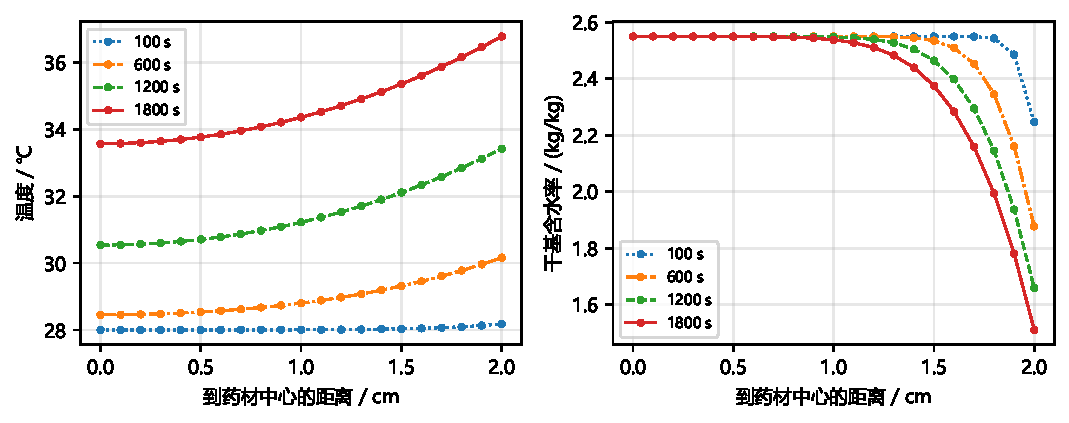
\includegraphics[width=\textwidth]{fig1_p1_profile}
\caption{问题 1 的温度与干基含水率径向分布}
\label{fig:p1}
\end{figure}

\begin{table}[htbp]
\centering
\caption{问题 1：预热阶段药材温度（单位：$^\circ$C）}
\label{table_01_p1_temperature}
\begin{tabular}{cccccc}
\toprule
时间 / s & 0.0 & 0.5 & 1.0 & 1.5 & 2.0 \\
\midrule
100 & 28.0001 & 28.0004 & 28.0041 & 28.0328 & 28.1801 \\
300 & 28.0409 & 28.0636 & 28.1515 & 28.3682 & 28.8489 \\
600 & 28.4535 & 28.5362 & 28.8041 & 29.3160 & 30.1653 \\
900 & 29.3245 & 29.4584 & 29.8756 & 30.6163 & 31.7305 \\
1200 & 30.5429 & 30.7099 & 31.2225 & 32.1127 & 33.4277 \\
1500 & 31.9959 & 32.1869 & 32.7662 & 33.7464 & 35.1203 \\
1800 & 33.5755 & 33.7721 & 34.3643 & 35.3622 & 36.7856 \\
\bottomrule
\end{tabular}
\end{table}

\begin{table}[htbp]
\centering
\caption{问题 1：预热阶段药材干基含水率（单位：kg/kg）}
\label{table_02_p1_moisture}
\begin{tabular}{cccccc}
\toprule
时间 / s & 0.0 & 0.5 & 1.0 & 1.5 & 2.0 \\
\midrule
100 & 2.5500 & 2.5500 & 2.5500 & 2.5500 & 2.2471 \\
300 & 2.5500 & 2.5500 & 2.5500 & 2.5492 & 2.0509 \\
600 & 2.5500 & 2.5500 & 2.5500 & 2.5353 & 1.8770 \\
900 & 2.5500 & 2.5500 & 2.5497 & 2.5045 & 1.7547 \\
1200 & 2.5500 & 2.5500 & 2.5482 & 2.4646 & 1.6586 \\
1500 & 2.5500 & 2.5499 & 2.5445 & 2.4206 & 1.5787 \\
1800 & 2.5500 & 2.5497 & 2.5383 & 2.3755 & 1.5102 \\
\bottomrule
\end{tabular}
\end{table}


\section{问题 2：变物性完整烘干过程}

本问改用附录 3 的物性关系，$\rho$、$c_p$、$k$ 成为含水率的函数，$D$ 同时依赖含水率与温度，方程由拟线性转为完全非线性。预热平衡段与恒温干燥段的差别体现在边界条件上：$0\sim14400$\,s 直接采用附件 1 的实测值，其后按末次观测值（$50.165\,^\circ$C、$0.04986$\,kg/kg）保持恒定。这样两段之间自然连续，无需人为设定切换时刻。

3\,h 时温度场已接近均匀，中心 $49.8495\,^\circ$C 与表面 $49.9664\,^\circ$C 相差仅 $0.12$\,K，与烘房温度一致，说明预热平衡已经完成；含水率仍保持明显径向梯度，中心 $1.7662$\,kg/kg、表面 $1.0081$\,kg/kg（图~\ref{fig:p2}、表~\ref{table_03_p2_temperature}、\ref{table_04_p2_moisture}）。

与问题 1 相比，同样时间内水分变化剧烈得多（中心由 $2.55$ 降到 $1.77$，而问题 1 的 30\,min 内中心毫无变化）。原因有两个：温度升到 $50\,^\circ$C 后 $e^{-3850/T_K}$ 放大，扩散加快；附录 3 的 $D$ 随含水率下降的衰减速度明显慢于附录 2，从高含水率到低含水率，附录 2 的 $D$ 下降约 265 倍，附录 3 只下降约 17 倍。

\begin{figure}[htbp]
\centering
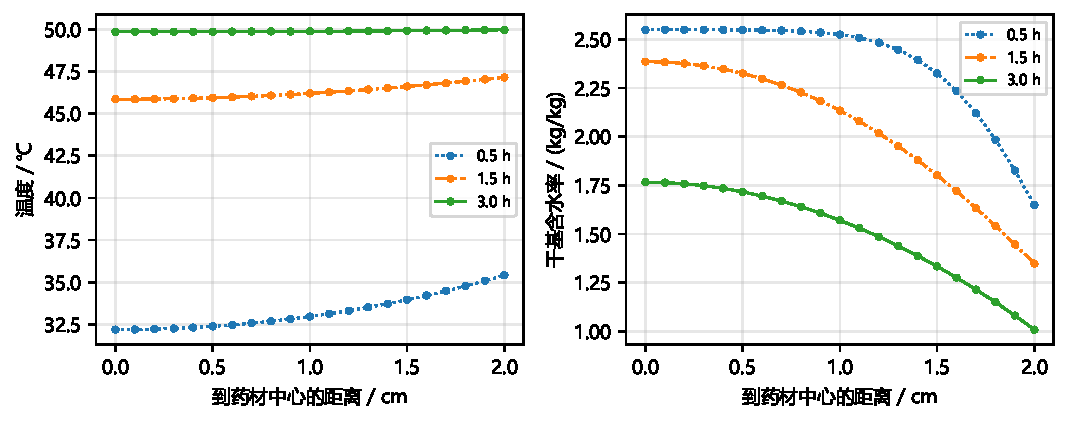
\includegraphics[width=\textwidth]{fig2_p2_profile}
\caption{问题 2 的温度与干基含水率径向分布}
\label{fig:p2}
\end{figure}

\input{tables/table_03_p2_temperature}
\input{tables/table_04_p2_moisture}

\section{问题 3：固定半径下的烘干时长}

在同一模型上持续推进，直到全场含水率低于 $0.15$\,kg/kg。结果为
\begin{equation}
t_3 = 57.21\ \text{h}\ (=2.38\ \text{天}).
\end{equation}

过程呈现明显的长尾：中心含水率由 $2.55$ 降到 $0.30$ 只用了 18\,h，剩下的 $0.15$ 又用了 39\,h。原因在 $D_{2,3}$ 的 $e^{-0.45/C}$ 项，含水率越低衰减越剧烈，$C$ 由 1 降到 0.15 时该项下降十余倍，扩散接近停滞。表面在 12.6\,h 就已降到 $0.15$ 以下，中心则一直拖到最后。表~\ref{table_05_p3_moisture} 与图~\ref{fig:p3}(a) 给出结果。

该时长与题干所述的"烘干过程一般持续 2$\sim$3 天"一致，是模型量级正确的一个旁证。

\begin{figure}[htbp]
\centering
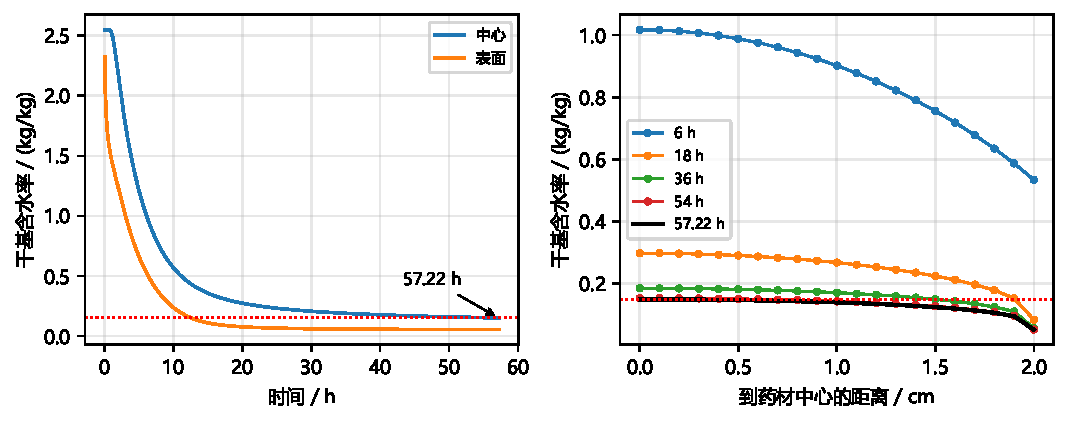
\includegraphics[width=\textwidth]{fig3_p3}
\caption{问题 3：中心与表面含水率演化（左）与各时刻径向剖面（右）}
\label{fig:p3}
\end{figure}

\input{tables/table_05_p3_moisture}

\section{问题 4：考虑收缩的烘干时长}

本问改用附录 4 的物性关系，半径按附件 2 的实测序列由 $2.000$\,cm 收缩到 $1.198$\,cm，计算域随之缩小。按第 4.3 节的物质坐标处理，得
\begin{equation}
t_4 = 50.86\ \text{h}\ (=2.12\ \text{天}),\qquad R(t_4)=1.200\ \text{cm}.
\end{equation}

表~\ref{table_06_p4_moisture} 中各列按当前时刻到药材中心的距离给出，最后一列是当前表面（图~\ref{fig:p4}）。由于半径在 3.64\,h 已缩到 $1.5$\,cm 以下，$1.5$\,cm 一列在该时刻之后落到药材之外，按题目"药材内部水分浓度"的表述留空。若改按材料点标注，表头应写成各点的初始位置，两套口径的中间几列数值不同，不宜混用。

收缩的影响需要与物性变化分开考察。问题 3 与问题 4 同时改变了物性公式和几何，两者之差不能直接解释为收缩效应。在同一物性（附录 4）下作对照：
\begin{equation}
\text{无收缩 }129.14\ \text{h}\ \longrightarrow\ \text{含收缩 }50.86\ \text{h},
\end{equation}
即收缩把烘干时间缩短到 $0.39$ 倍，提速 $2.54$ 倍。收缩使扩散路径由 $2.0$\,cm 降到 $1.198$\,cm，特征时间按 $(2/1.198)^2=2.79$ 倍缩短，与实测提速倍数吻合。

这一对照也解释了为什么问题 4 必须做动边界：若沿用固定半径，附录 4 的物性会给出 $5.4$ 天，与题干"2$\sim$3 天"直接矛盾。

\begin{figure}[htbp]
\centering
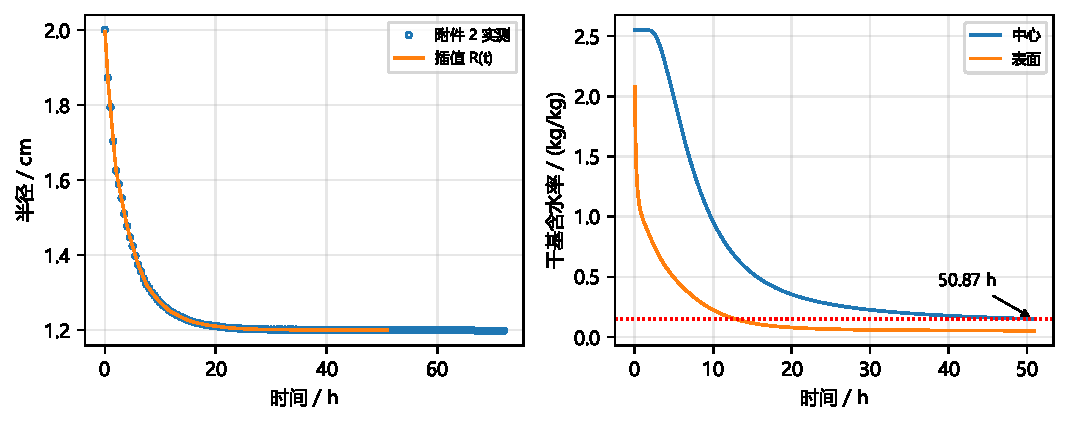
\includegraphics[width=\textwidth]{fig4_p4}
\caption{问题 4：半径路径与附件 2 实测值的比较（左）、中心与表面含水率演化（右）}
\label{fig:p4}
\end{figure}

\input{tables/table_06_p4_moisture}

\section{模型检验与灵敏度分析}

\subsection{网格与时间步收敛}

以问题 1 在 1800\,s 的解为对象，同时对空间和时间加密。相邻两级之间温度的最大偏差依次为 $4.90\times10^{-4}$、$2.72\times10^{-4}$、$1.43\times10^{-4}$、$7.32\times10^{-5}$、$3.70\times10^{-5}$\,K，比值稳定在 $0.5$ 附近；温度收敛阶估计为 $0.85$、$0.93$、$0.97$、$0.98$，逐级趋近一阶，与"一阶时间 $+$ 一阶空间"的格式相符。生产设置（640 层、$0.1$\,s）与参考设置（640 层、$0.03125$\,s）的偏差为 $8.2\times10^{-5}$\,K 与 $6.0\times10^{-6}$\,kg/kg，远低于四位小数要求（图~\ref{fig:ver}(a)）。

问题 3 的烘干时长对空间网格的收敛过程为：$N=20$ 时 $56.23$\,h，$40$ 时 $56.76$，$80$ 时 $57.02$，$160$ 时 $57.14$，$320$ 时 $57.19$，$640$ 时 $57.21$。相邻差值依次为 $0.53$、$0.26$、$0.12$、$0.05$\,h，每加密一倍减半。这组数据说明 $N=20$ 的结果尚未进入收敛区间，也说明生产网格已经足够。需要指出，烘干时长本身存在约 $0.3$\,h 的数值不确定度：结束前中心含水率每小时只降约 $0.001$\,kg/kg，含水率 $10^{-4}$ 的差异即对应约 $0.1$\,h，因此该时间报至 $0.1$\,h 量级即可。

\subsection{守恒性与解析解对比}

离散格式的守恒性可逐项核验。以初始状态为基准，内部焓的变化应等于表面热通量的时间积分，干物质含水量的变化应等于表面传质通量的时间积分。实测相对残差为能量 $2.7\times10^{-12}$、水分 $3.4\times10^{-13}$，说明通量在界面上严格抵消。

取环境温度恒为 $50\,^\circ$C、物性为常数，模型退化为经典的圆柱非稳态导热问题，其分离变量级数解可作基准。数值解与之的最大偏差在细网格上为 $2.5\times10^{-4}$\,K，在生产网格上为 $3.9\times10^{-4}$\,K，而整个过程温升为 $22$\,K，相对误差约 $10^{-5}$。这一项同时确认了空间离散与时间步长均已足够。

\subsection{界面系数平均方式的收敛对照}
\label{sec:face}

有限体积法界面上的传导率可以取算术平均，也可以取调和平均。两种规则都是相容格式，网格加密后必须收敛到同一结果；但在强非线性区（表面含水率已很低、$D$ 掉到 $10^{-12}$ 量级）粗网格上的差异很大，容易把网格误差误读为物理效应。为此对"平均方式 $\times$ 网格层数 $\times$ 传质口径"做了完整对照，结果见表~\ref{tab:face}。

\begin{table}[htbp]
\centering
\caption{界面系数平均方式与网格层数的收敛对照（问题 3 烘干时长，单位 h）}
\label{tab:face}
\begin{tabular}{ccccc}
\toprule
网格层数 & $km{=}1$ 算术 & $km{=}1$ 调和 & $km{=}820$ 算术 & $km{=}820$ 调和 \\
\midrule
320 & 57.190 & 57.617 & 53.140 & 174.75 \\
640 & 57.211 & 57.290 & 53.200 & 106.42 \\
1280 & 57.218 & 57.236 & 53.227 & 75.06 \\
2560 & 57.221 & 57.225 & 53.240 & 61.55 \\
\bottomrule
\end{tabular}
\end{table}

$km=1$ 时两种平均在 2560 层收敛到同一个值 $57.22$\,h，本文生产用的算术平均在 640 层即为 $57.21$\,h，已落在收敛值上，偏差 $0.02\%$。$km=820$ 的调和平均在 320 层给出 $174.75$\,h，随网格加密单调下降到 $61.55$\,h，朝算术平均的 $53.24$\,h 靠拢，属未收敛的中间结果。这组对照说明：比较两种离散格式之前必须确认两边都已收敛，否则网格误差会被当作物理效应；本文的传质口径灵敏度必须在收敛口径下计算。

\subsection{传质口径灵敏度}

题目给出的含水率是干基含水率（相对干物料），而空气水分浓度是绝对湿度（相对干空气），两者基准不同。边界式
\[
-D\frac{\partial C}{\partial r}=k_m\left[C(R,t)-C_\infty\right]
\]
相当于把空气侧的湿度按与药材含水率同一口径处理，是本题可用的最小假设；严格换算需要吸附等温线与干物质密度，题目未给。为判断该假设的影响，引入无量纲系数 $\kappa$，令有效传质系数为 $\kappa h_m$，结果见表~\ref{tab:km} 与图~\ref{fig:ver}(b)。

\begin{table}[htbp]
\centering
\caption{传质口径灵敏度（问题 3 烘干时长）}
\label{tab:km}
\begin{tabular}{ccccc}
\toprule
$\kappa$ & 0.1 & 1（基线） & 10 & 820 \\
\midrule
表面降到 $0.15$ 的时刻 / h & 110.1 & 12.6 & 2.5 & 0.0 \\
整体降到 $0.15$ 的时刻 / h & 144.5 & 57.2 & 53.2 & 53.2 \\
24\,h 时中心含水率 / (kg/kg) & 1.37 & 0.24 & 0.21 & 0.21 \\
\bottomrule
\end{tabular}
\end{table}

把口径放大到内扩散控制极限，烘干时长只由 $57.2$\,h 降到 $53.2$\,h（$-7\%$），且 $\kappa\ge10$ 后已经饱和，说明内部扩散始终是主控环节，外边界阻力并非瓶颈。反过来，口径缩小到 $0.1$ 时外部传质成为瓶颈，24\,h 时中心含水率仍有 $1.37$\,kg/kg，整体需要 $144.5$\,h，与题干区间矛盾。因此题目给定的 $h_m=8\times10^{-7}$\,m/s 取值落在唯一能与"2$\sim$3 天"自洽的区间内，模型对口径放大的方向不敏感。

\subsection{蒸发潜热的量级审计}
\label{sec:latent}

主模型未向能量方程叠加蒸发潜热项。这一简化是否成立，可作量级审计：在 1800\,s，表面含水率 $1.5102$\,kg/kg、空气水分浓度 $0.0331$\,kg/kg，按题给传质系数得界面通量（以含水率口径计）$1.18\times10^{-6}$\,kg/(kg$\cdot$s)；若分别按表观密度 $820$\,kg/m$^3$ 和干物质密度 $231$\,kg/m$^3$ 折算为质量通量，再乘以水的汽化潜热 $2.257\times10^{6}$\,J/kg，得潜热汇约 $2187$\,W/m$^2$ 与 $616$\,W/m$^2$；同一时刻对流供热为 $h(T_\infty-T_s)=118$\,W/m$^2$。潜热需求是对流供热的 $5.2\sim18.5$ 倍，取决于密度口径。

这说明题给的热、质边界是分别标定的等效闭合，不能与潜热项机械拼合：一旦叠加，表面会在远低于空气温度处达到能量平衡，模型将由内部扩散控制转为供热控制，与题干给出的时间尺度不符。严格的潜热耦合需要干物质密度、气固平衡含水率关系与有效汽化潜热，题目均未提供，故本文将其列为扩展模型。

\subsection{两阶段切换点与收缩效应}

预热平衡段与恒温干燥段的划分方式可作检验。把切换点显式取在 1.5\,h、2\,h、4\,h 三种位置重新计算，烘干时长均为 $57.58$\,h，与默认的连续边界处理（$57.21$\,h）相差 $0.6\%$，说明切换判据不敏感。

收缩与物性变化的分离见第 9 节：在附录 4 物性下，无收缩为 $129.14$\,h，含收缩为 $50.86$\,h，收缩使时间缩短约 $61\%$；而问题 3 到问题 4 的净变化仅 $-11\%$，因为物性变化使时间延长了 $2.26$ 倍，与收缩的缩短作用部分抵消。把两者混在一起讨论会严重低估收缩的作用。

\begin{figure}[htbp]
\centering
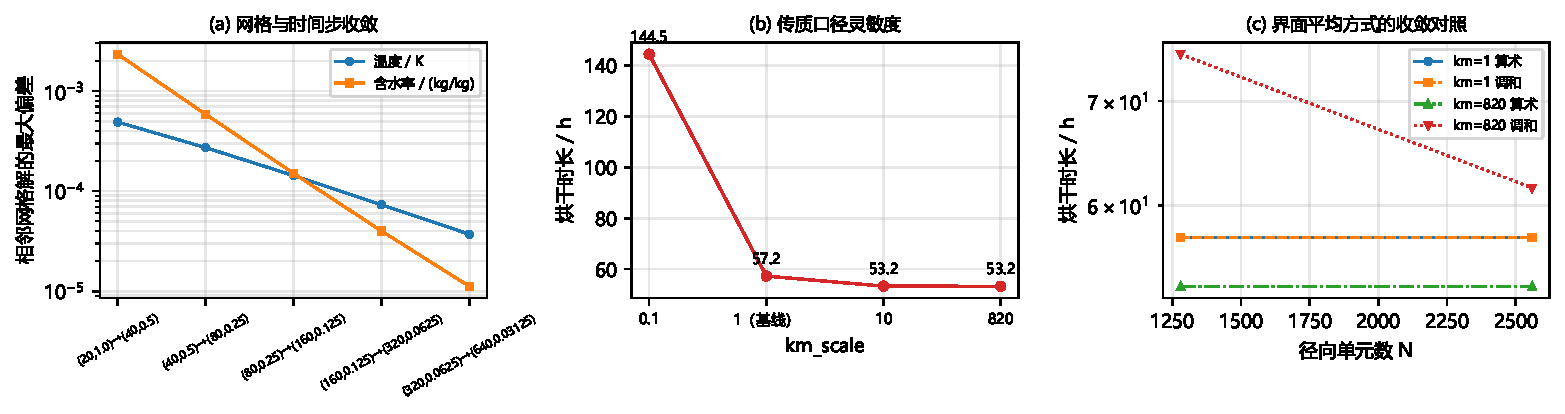
\includegraphics[width=\textwidth]{fig5_verification}
\caption{模型检验：(a) 网格与时间步收敛；(b) 传质口径灵敏度；(c) 界面系数平均方式的收敛对照}
\label{fig:ver}
\end{figure}

\section{模型评价与改进方向}

\subsection{模型优点}

模型直接由守恒定律导出，各项物理含义明确；有限体积离散在柱坐标下保持守恒，中心奇异性自然消除，且同一套代码通过替换物性函数即可覆盖四个问题；问题 4 采用物质坐标，避免动网格重构，半径缩小时节点值不发生虚假跳变；模型对网格、时间步、界面平均方式与两阶段切换点均作了收敛或敏感性检验，结论不依赖离散细节。

\subsection{模型局限}

第一，恒温干燥段的空气温湿度由附件 1 的末值外推，附件 1 只覆盖 4\,h，这是模型最主要的外部不确定性来源；改用平台段均值只使烘干时长变化 $0.6\%$，但若实际工艺另有设定值则需重算。第二，模型未显式耦合蒸发潜热，理由见第~\ref{sec:latent} 节，这限制了它在供热受限工况下的适用性。第三，水分迁移简化为单一有效扩散，未区分液态迁移与蒸汽扩散，也未考虑表面结壳与各向异性。第四，附件 2 的半径在约 20\,h 后基本停止收缩，而含水率要到约 57\,h 才达标，实测收缩快于失水，说明该序列由外部标定，不宜反过来作为失水的验证量。第五，问题 2 结果文件的时间范围在题目中存在两种读法（前 3\,h 或整个烘干过程），本文同时提供两份结果。

\section{结论}

本文建立了圆柱药材热风干燥的一维径向热湿传递模型，并用守恒有限体积法求解四个问题。

\begin{enumerate}
\item 预热 1800\,s 时中心与表面温度分别为 $33.5755\,^\circ$C 与 $36.7856\,^\circ$C，干基含水率为 $2.5500$ 与 $1.5102$\,kg/kg；水分变化集中在距表面约 $5$\,mm 的薄层内。
\item 采用附录 3 变物性后，3\,h 时温度场接近均匀（中心 $49.8495\,^\circ$C、表面 $49.9664\,^\circ$C），含水率仍保持径向梯度（中心 $1.7662$、表面 $1.0081$\,kg/kg）。
\item 固定半径下烘干时长为 $57.21$\,h；网格加密到 2560 层后收敛到 $57.22$\,h，算术与调和两种界面平均方式给出同一结果。
\item 计入附件 2 的收缩路径后烘干时长为 $50.86$\,h，结束时半径约 $1.200$\,cm；在同一物性下，收缩使烘干时间缩短约 $61\%$，是决定结果量级的关键因素。
\end{enumerate}

\begin{thebibliography}{9}
\bibitem{incropera} Incropera F P, DeWitt D P, Bergman T L, et al. \emph{Fundamentals of Heat and Mass Transfer}. 7th ed. Hoboken: John Wiley \& Sons, 2011.
\bibitem{carslaw} Carslaw H S, Jaeger J C. \emph{Conduction of Heat in Solids}. 2nd ed. Oxford: Clarendon Press, 1959.
\bibitem{patankar} Patankar S V. \emph{Numerical Heat Transfer and Fluid Flow}. New York: Hemisphere Publishing, 1980.
\bibitem{crank} Crank J. \emph{The Mathematics of Diffusion}. 2nd ed. Oxford: Clarendon Press, 1975.
\end{thebibliography}

\appendix
\section{程序与结果文件说明}

全部计算由 Python 完成，代码与结果文件的对应关系如下：

\begin{itemize}
\item \texttt{src/config.py}：几何与附录 2 参数、数值配置；
\item \texttt{src/preprocess.py}：附件 1、2 的质量检查与分段线性插值；
\item \texttt{src/fv.py}：节点中心有限体积求解器，支持动边界与两种界面平均方式；
\item \texttt{src/props.py}：附录 3、4 的经验关系；
\item \texttt{src/run\_p1.py}、\texttt{src/run\_p234.py}：四个问题的主程序；
\item \texttt{src/verify\_p1.py}：收敛性、守恒性与解析解校验；
\item \texttt{src/convergence\_face\_avg.py}、\texttt{src/convergence\_extreme.py}：界面平均方式的收敛对照；
\item \texttt{src/sens\_km.py}：传质口径灵敏度；
\item \texttt{output/result1.xlsx}$\sim$\texttt{result4.xlsx}：题目要求的结果文件；
\item \texttt{logs/}：各次检验的原始数据（JSON）。
\end{itemize}

程序只读取题目附件，不在运行过程中修改原始数据；随机性不参与计算，结果可完全复现。

\end{document}
